%%%%%%%%%%%%%%%%%%%%%%%%%%%%%%%%%%%%%%%%%%%%%%%%%%%%%%%%%%%
% --------------------------------------------------------
% Tau
% LaTeX Template
% Version 2.4.4 (28/02/2025)
%
% Author:
% Guillermo Jimenez (memo.notess1@gmail.com)
%
% License:
% Creative Commons CC BY 4.0
% --------------------------------------------------------
%%%%%%%%%%%%%%%%%%%%%%%%%%%%%%%%%%%%%%%%%%%%%%%%%%%%%%%%%%%

\documentclass[9pt,a4paper,twocolumn,twoside]{tau-class/tau}
\usepackage[english]{babel}

%% Spanish babel recomendation
% \usepackage[spanish,es-nodecimaldot,es-noindentfirst]{babel}

%% Draft watermark
% \usepackage{draftwatermark}

%----------------------------------------------------------
% TITLE
%----------------------------------------------------------

\journalname{Lotus Valley International School Gurugram}
\title{Valtam: a bot to solve student troubles}

%----------------------------------------------------------
% AUTHORS, AFFILIATIONS AND PROFESSOR
%----------------------------------------------------------

\author[a]{Jayan Sunil}
\author[b]{Rachit Rustagi}
\author[c]{Aarav Khandpur}

%----------------------------------------------------------

\affil[a]{IX --- Everest, +91 9910856655}
\affil[b]{IX --- Nilgiris, +91 9211450648}
\affil[c]{IX --- Nilgiris, +91 9211612568}

\professor{}

%----------------------------------------------------------
% FOOTER INFORMATION
%----------------------------------------------------------

\institution{Valtam}
\footinfo{Lotus Valley International School Gurugram}
\theday{\today}
\leadauthor{Jayan et al.}
\course{Shiv Nadar Interschool Competition}

%----------------------------------------------------------
% ABSTRACT AND KEYWORDS
%----------------------------------------------------------

\begin{abstract}
	This project, Valtam, is a chatbot that is designed to solve the most frustrating that students face in their daily lives. From struggling to find assignments to needing help with their cumbersome homeworks, this chatbot can do it all --- all while being reliable and easy to use.
\end{abstract}

%----------------------------------------------------------

\keywords{\url{shiv-nadar.vercel.app}}

%----------------------------------------------------------

\begin{document}

\maketitle
\thispagestyle{firststyle}
\tauabstract
\tableofcontents
\linenumbers

%----------------------------------------------------------

\section{Introduction}

\taustart{W}elcome to Valtam, the chatbot to solve it all. This bot is designed to fulfil your every need as a student: it can find your homework, and it can help you solve it. Utilizing modern frameworks, the bot entails a clean, functional UI, making the power of Python accessible to the layperson. This document is a guide to the inner working of Valtam.


\section{Technologies Used}
\begin{enumerate}
	\item NextJS (frontend)
	      \begin{itemize}
		      \item Shadcn/ui (UI)
		      \item Better Auth (User Authentication)
	      \end{itemize}
	\item Python (backend)
	      \begin{itemize}
		      \item API calls --- FastAPI
		      \item LLM --- PyTorch and Transformers (HuggingFace)
	      \end{itemize}
	\item PostgreSQL (database)
	      \begin{itemize}
		      \item ORM --- Drizzle
		      \item DB provider --- Vercel Postgres (Neon)
	      \end{itemize}
	\item Telemery and Analytics
	      \begin{itemize}
		      \item Telemetry \& Error Reporting --- Sentry
		      \item Analytics --- Posthog
	      \end{itemize}
\end{enumerate}
\subsection{Frontend}
For a fast and responsive frontend, we used NextJS. Its vast ecosystem, and reliability were major perks. It allowed us to create many complex functions effectively. To make NextJS even better, we used Shadcn, a popular UI library that provides accesible base components. For authentication, we used BetterAuth, an open-source authentication library that gives us support for many social logins like Google and Github.

\subsection{Backend \& Database}
backend has two parts: the LLM and the API. The LLM is powered by PyTorch and Transformers, where we have trained a base model to cater to a student's needs. There are two trained models: one that is only for the NCERT and one that also has the assignments. To allow the frontend to interact with the LLM, we have a FastAPI wrapper around the model. The API has two routes: \verb|/generate/{ncert,assignments}|, which take a request body of \begin{lstlisting}[language=TeX, caption=Request Body for /generate/*]
	{
		prompt: string;
		temperature: number (defaults to 0.7);
		max_length: number (defaults to 128);
	}
\end{lstlisting}
\subsection{Model}
To ensure that our chatbot is relevant to the academic context of Indian school students, we fine-tuned the LLM using a dataset of NCERT textbook explanations. We used two publicly available NCERT-based datasets for \href{https://huggingface.co/datasets/KadamParth/NCERT_Science_9th}{Science} and \href{https://huggingface.co/datasets/KadamParth/NCERT_Social_Studies_9th}{Social Science} with approximately 8k rows on 3 epochs.

We chose the Qwen 0.6B model for this project.

The training pipeline used the NCERT Database combined with a database which has queries from our school portal
\begin{itemize}
	\item \textbf{Tokenizer:} AutoTokenizer from Qwen model
	\item \textbf{Max Length:} 128 tokens
	\item \textbf{Epochs:} 3
	\item \textbf{Precision:} FP16 (mixed-precision training)
\end{itemize}

We used PyTorch for low-level control and trained the model locally on our GPU. After training, the model showed improved performance on curriculum-specific queries, demonstrating a solid understanding of academic content.

\subsection{More Information}

The bot's main use case is supposed to be in QA format(Question-Answering), as it is supposed to answer queries and provide help to students Therefore, the data was organised into a Question-Answer format for optimal training. The Qwen 0.6B (752M params) model offers speed, balance and accuracy. To training this model, we used an RTX 4070 GPU on a machine with the following specs.
\begin{itemize}
	\item CPU: i5-13500k
	\item RAM: 16GB
	\item GPU: RTX 4070
	\item Storage: 1TB NVME 4.0 SSD
\end{itemize} For the model with only the NCERT, the training loss metric is shown in Table \ref{tab:train_loss}.
\begin{table}[H]
	\centering
	\caption{Training Loss for model 1:}
	\label{tab:train_loss}
	\begin{tabular}{ll}
		\toprule
		\textbf{Step} & \textbf{Training Loss} \\
		\midrule
		500           & 1.312500               \\
		1000          & 0.921400               \\
		1500          & 0.623400               \\
		2000          & 0.291200               \\
		2500          & 0.202200               \\
		3000          & 0.155800               \\
		3500          & 0.109400               \\
		4000          & 0.069900               \\
		4500          & 0.059500               \\
		\bottomrule
	\end{tabular}
\end{table}


The database is a PostgreSQL database, which is used to store user information and their chat history. We use Vercel Postgres, with Neon, for a fast and scalable experience. As the ORM, we use Drizzle, which is type-safe, lightweight, and has a SQL-centric approach to interacting with databases, making it ideal for modern TypeScript.

\begin{figure}[h]
	\centering
	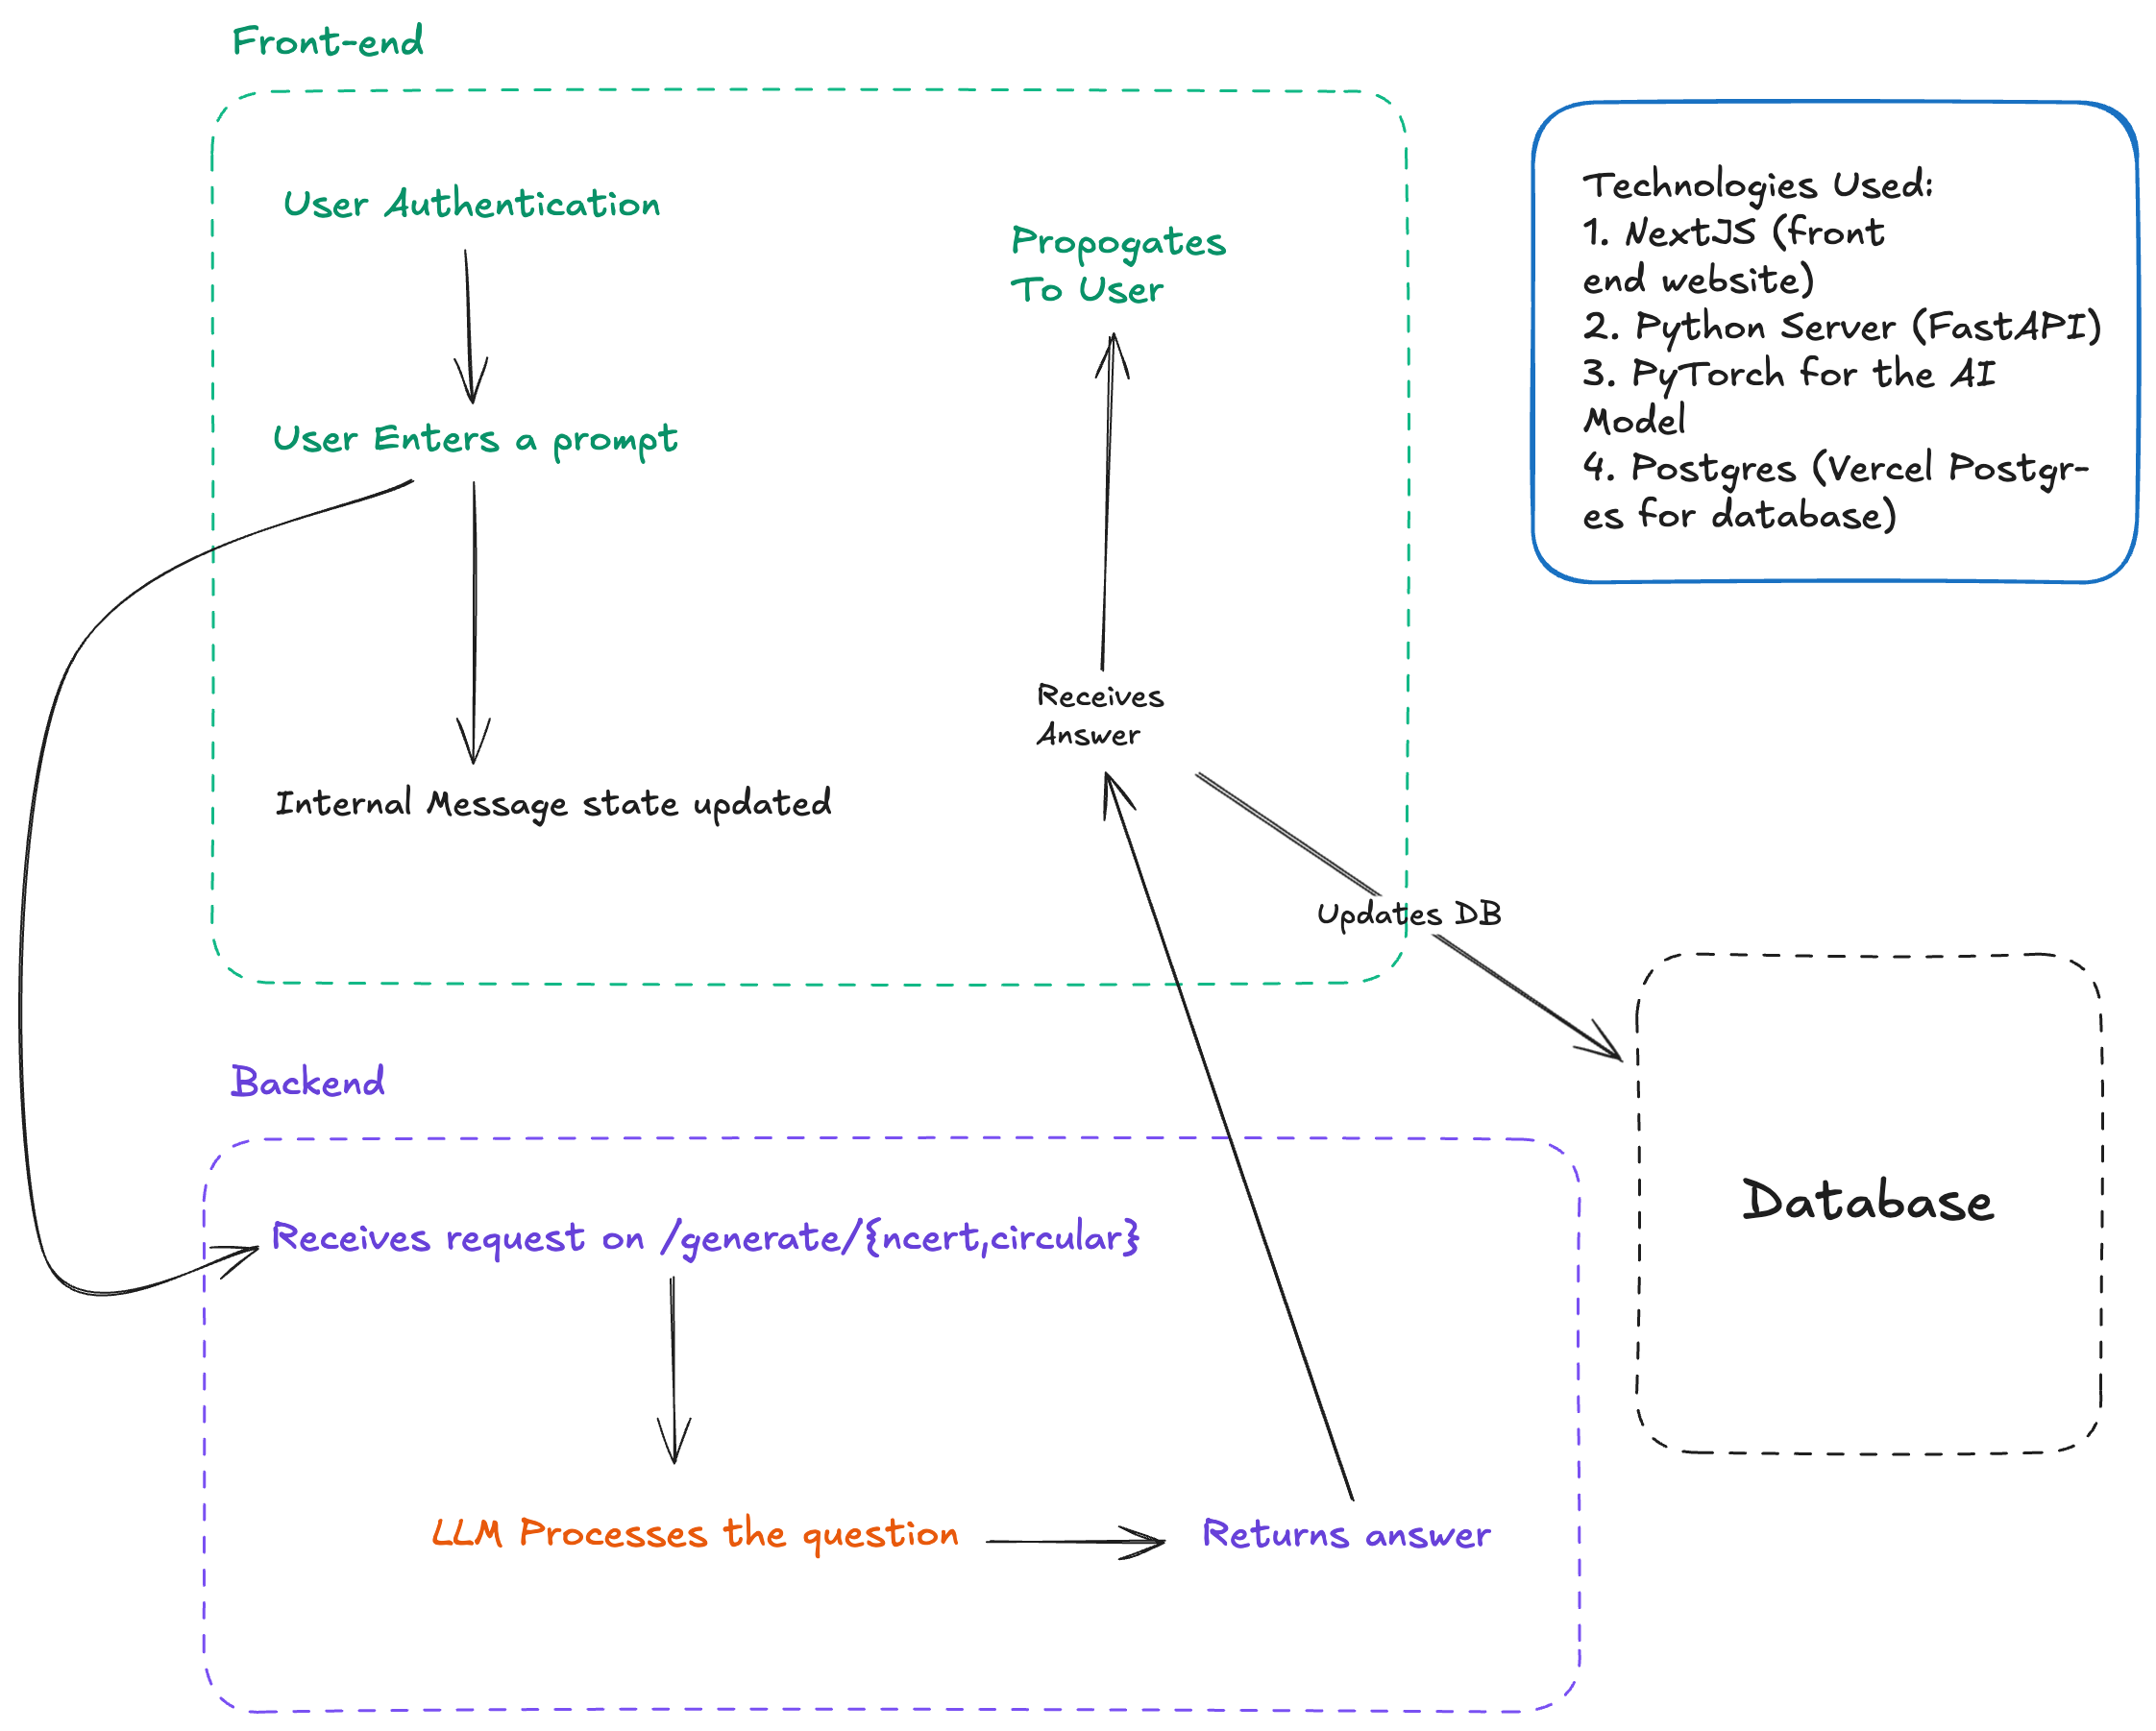
\includegraphics[width=2\linewidth]{./flow-chart.png}
	\caption{A flow chart of the application lifecycle.}
	\label{fig:1}
\end{figure}
\end{document}
